%
% This is the LaTeX template file for lecture notes for EE 382C/EE 361C.
%
% To familiarize yourself with this template, the body contains
% some examples of its use.  Look them over.  Then you can
% run LaTeX on this file.  After you have LaTeXed this file then
% you can look over the result either by printing it out with
% dvips or using xdvi.
%
% This template is based on the template for Prof. Sinclair's CS 270.

\documentclass[twoside]{article}
\usepackage{graphics}
\usepackage{float}
\usepackage{tikz}
\usepackage{listings}
\usepackage{graphicx}
\setlength{\oddsidemargin}{0.25 in}
\setlength{\evensidemargin}{-0.25 in}
\setlength{\topmargin}{-0.6 in}
\setlength{\textwidth}{6.5 in}
\setlength{\textheight}{8.5 in}
\setlength{\headsep}{0.75 in}
\setlength{\parindent}{0 in}
\setlength{\parskip}{0.1 in}

%
% The following commands set up the lecnum (lecture number)
% counter and make various numbering schemes work relative
% to the lecture number.
%
\newcounter{lecnum}
\renewcommand{\thepage}{\thelecnum-\arabic{page}}
\renewcommand{\thesection}{\thelecnum.\arabic{section}}
\renewcommand{\theequation}{\thelecnum.\arabic{equation}}
\renewcommand{\thefigure}{\thelecnum.\arabic{figure}}
\renewcommand{\thetable}{\thelecnum.\arabic{table}}

%
% The following macro is used to generate the header.
%
\newcommand{\lecture}[4]{
   \pagestyle{myheadings}
   \thispagestyle{plain}
   \newpage
   \setcounter{lecnum}{#1}
   \setcounter{page}{1}
   \noindent
   \begin{center}
   \framebox{
      \vbox{\vspace{2mm}
    \hbox to 6.28in { {\bf EE 382C/361C: Multicore Computing
                        \hfill Fall 2016} }
       \vspace{4mm}
       \hbox to 6.28in { {\Large \hfill Lecture #1: #2  \hfill} }
       \vspace{2mm}
       \hbox to 6.28in { {\it Lecturer: #3 \hfill Scribe: #4} }
      \vspace{2mm}}
   }
   \end{center}
   \markboth{Lecture #1: #2}{Lecture #1: #2}
   %{\bf Disclaimer}: {\it These notes have not been subjected to the
   %usual scrutiny reserved for formal publications.  They may be distributed
   %outside this class only with the permission of the Instructor.}
   \vspace*{4mm}
}

%
% Convention for citations is authors' initials followed by the year.
% For example, to cite a paper by Leighton and Maggs you would type
% \cite{LM89}, and to cite a paper by Strassen you would type \cite{S69}.
% (To avoid bibliography problems, for now we redefine the \cite command.)
% Also commands that create a suitable format for the reference list.
\renewcommand{\cite}[1]{[#1]}
\def\beginrefs{\begin{list}%
        {[\arabic{equation}]}{\usecounter{equation}
         \setlength{\leftmargin}{2.0truecm}\setlength{\labelsep}{0.4truecm}%
         \setlength{\labelwidth}{1.6truecm}}}
\def\endrefs{\end{list}}
\def\bibentry#1{\item[\hbox{[#1]}]}

%Use this command for a figure; it puts a figure in wherever you want it.
%usage: \fig{NUMBER}{SPACE-IN-INCHES}{CAPTION}
\newcommand{\fig}[3]{
			\vspace{#2}
			\begin{center}
			Figure \thelecnum.#1:~#3
			\end{center}
	}
% Use these for theorems, lemmas, proofs, etc.
\newtheorem{theorem}{Theorem}[lecnum]
\newtheorem{lemma}[theorem]{Lemma}
\newtheorem{proposition}[theorem]{Proposition}
\newtheorem{claim}[theorem]{Claim}
\newtheorem{corollary}[theorem]{Corollary}
\newtheorem{definition}[theorem]{Definition}
\newenvironment{proof}{{\bf Proof:}}{\hfill\rule{2mm}{2mm}}

% **** IF YOU WANT TO DEFINE ADDITIONAL MACROS FOR YOURSELF, PUT THEM HERE:

\begin{document}
%FILL IN THE RIGHT INFO.
%\lecture{**LECTURE-NUMBER**}{**DATE**}{**LECTURER**}{**SCRIBE**}
\lecture{18}{November 27}{Vijay Garg}{Huy Doan}
%\footnotetext{These notes are partially based on those of Nigel Mansell.}


% **** YOUR NOTES GO HERE:

% Some general latex examples and examples making use of the
% macros follow.  
%**** IN GENERAL, BE BRIEF. LONG SCRIBE NOTES, NO MATTER HOW WELL WRITTEN,
%**** ARE NEVER READ BY ANYBODY.
\section{Atomic Scan}
Scan $\rightarrow$ atomic read of multiple locations
Update $\rightarrow$ atomic write of a single location

\textbf{Scenario: } Assume SWSR and the memory as follow

\begin{figure}[H]
    \centering
    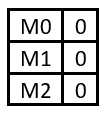
\includegraphics{initialmemory.png}
    \caption{Initial Memory}
    \label{fig:1}
\end{figure}

We are doing two operations W(M0,1), W(M1,1) sequentially. The memory states M0M1M2 we expect to observe are 100, 110. However, a scan may result in the state 010. This result means that the scan operation is not linearizable.

\begin{figure}[H]
    \centering
    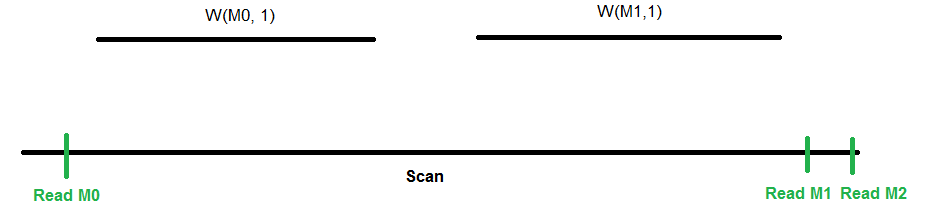
\includegraphics[scale=0.5]{scan.png}
    \caption{Bad Scan}
    \label{fig:2}
\end{figure}

\textbf{Solution: }\\
\textit{Update}\\
    Write the new value with the updated timestamp\\
\textit{Scan}\\
    Collect an entire array in W\\
    Loop:\\
        Read the entire array again to make sure that there is no change to the timestamp (2nd collect)\\
        If there is some change, go back to loop
        
$\rightarrow$ The algorithm is lock-free but not wait-free because if writes keep coming, scan has to loop and wait

\begin{figure}[H]
    \centering
    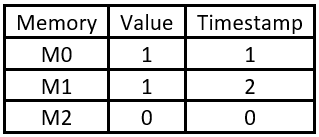
\includegraphics{timestamp.png}
    \caption{Memory with timestamp}
    \label{fig:3}
\end{figure}

\textbf{NOTE: } It is impossible to solve the dual problem which is write to multiple locations and read a single location in a wait-free manner.



\section{Consensus}

\begin{figure}[H]
    \centering
    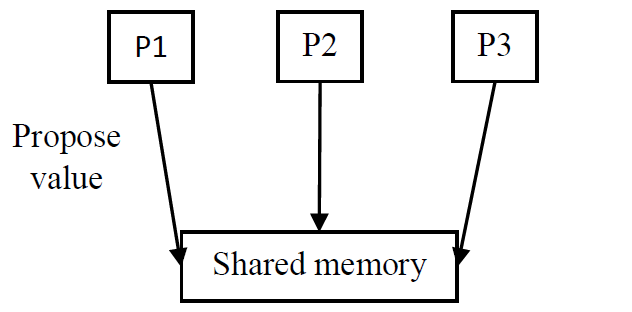
\includegraphics[scale=0.75]{sharedmemory.png}
    \caption{Consensus Problem}
    \label{fig:4}
\end{figure}

Consensus is a problem that requires a given set of processes to agree on an input value. As depicted in Figure 18.4, each process proposes its own value and the system has to decide which value among those that all processes will agree on.

The \textbf{requirements} on any object implementing consensus are as follows:
\begin{itemize}
    \item Agreement:  No two correct processes decide on different values.
    \item Validity: The value decided must be proposed by some process.
    \item Wait-freedom: Decides in a finite number of steps.
\end{itemize}



\subsection{Bully Algorithm}

Assume that we have two process P0 and P1 and no process fails. The propose values of P0 and P1 are stored in the array prop[2]. The bully algorithm solves the consensus problem by just simply picking prop[0] at all time.

\begin{center}
\renewcommand{\lstlistingname}{Consensus}
\begin{lstlisting}[language=Java, caption=Bully Algorithm, frame=single, basicstyle=\small]
Pi
    Write your proposal to the prop array
    Every process waits until prop[0] becomes non-null
    Decide on prop[0]
\end{lstlisting}
\end{center}

Obviously, this algorithm is not fair and not fault-tolerant in case that P0 fails.

\subsection{Global State Overview}
\textbf{Global State:} the state of the shared memory

Formally, let $G.V$ is the set of decision values reachable from global state $G$. We say G is \textbf{bivalent} if $|G.V| = 2$ and \textbf{univalent} if $|G.V| = 1$. In the latter case, we call $G$ $0-valent$ if $G.V = {0}$ and $G$ $1-valent$ if $G.V = {1}$. The bivalent state captures the notion of indecision.

A bivalent state is \textbf{critical} if any action by any process leads to a 0-valent or 1-valent state

\begin{figure}[H]
    \centering
    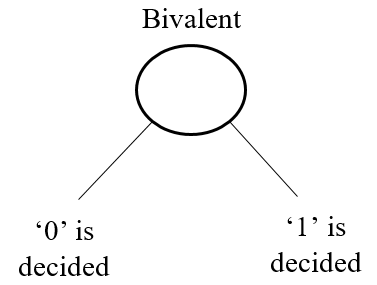
\includegraphics[scale=0.75]{bivalent.png}
    \caption{Bivalent State}
    \label{fig:5}
\end{figure}

\textbf{Claim 1}: There exists an initial bivalent global state for any consensus protocol.

\textbf{Proof:}
Consider the most simple case where there are only two processes. If P1 is slow and P0 runs solo, P0 will eventually decide on '0'. Similarly P1 can run solo and decide on '1'. Therefore, the initial state G is bivalent.

\begin{figure}[H]
    \centering
    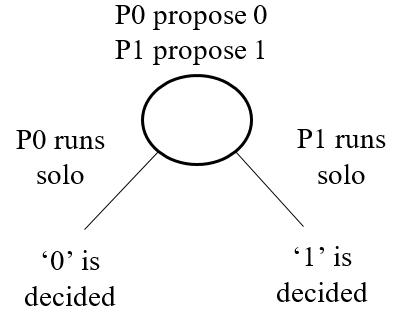
\includegraphics[scale=0.75]{firstclaim.png}
    \caption{Bivalent State of Two Processes}
    \label{fig:6}
\end{figure}

\textbf{Claim 2}: There exists a critical global state for every consensus protocol.

\subsection{Theorem}
It is impossible to solve consensus with just read and write.\\
\textbf{Proof:} We show that even in a two-process system, atomic registers cannot be used to go to non-bivalent states in a consistent manner. We perform a case analysis of events that can be done by two processes, say, P and Q in a critical state S. Let e be the event at P and event f be at Q be such that e(S) has a decision value different from that of f(S). 
We now do a case analysis:
\begin{itemize}
    \item Case 1: e and f are operations on different registers. We observe that ef(S) and fe(S) are identical and,  therefore, have the same decision value. However, we assume earlier that e(S) and f(S) have different decision values, which implies that e(f(S)) and f(e(S)) have different decision values since the decision values cannot change.
    \item Case 2: e is read and f is write. When P does e, the state of Q does not change. Therefore, f(S) and f(e(S)) are identical and have the same decision values.
    \item Case 3: e and f are write on the same registers. Obviously, f(S) and f(e(S)) are identical and have the same decision values.
\end{itemize}

\begin{figure}[H]
    \begin{minipage}{.3\textwidth}\centering
    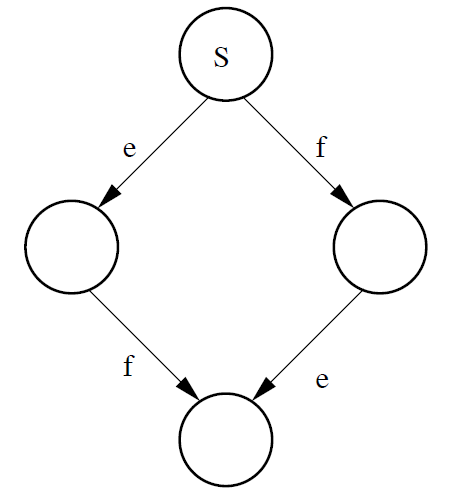
\includegraphics[scale=0.3]{case1.png}
    \caption{Case 1: e and fa are operations on different registers}
    \end{minipage}    
    \begin{minipage}{.3\textwidth}\centering
        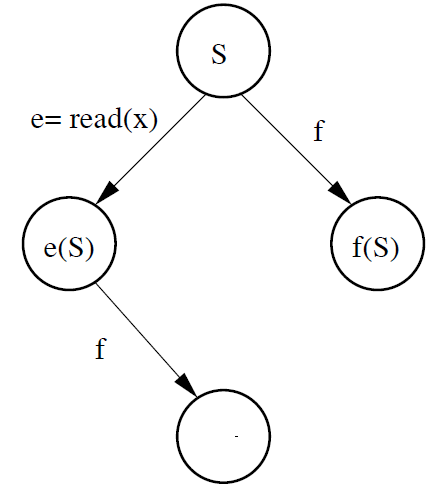
\includegraphics[scale=0.3]{case2.png}
    \caption{Case 2: one read one write}
    \end{minipage}    
    \begin{minipage}{.3\textwidth}\centering
    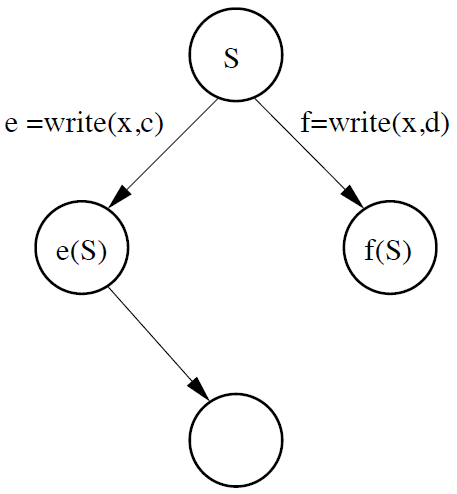
\includegraphics[scale=0.3]{case3.png}
    \caption{Case 3: two writes on the same register}
    \end{minipage}
    
    \label{fig:7}    
\end{figure}

\subsection{Consensus Number}
Consensus number of a shared object class O is the maximum number of processes that use object from class O to solve consensus

\begin{figure}[H]
    \centering
    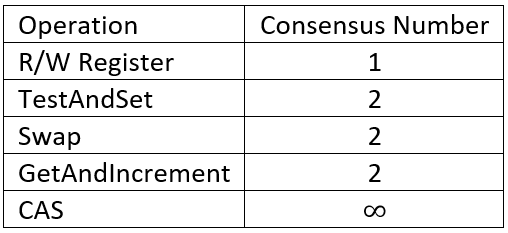
\includegraphics[scale=0.75]{consensusnumber.png}
    \caption{Consensus Number of Some Operations}
    \label{fig:10}
\end{figure}

\textbf{Queue has consensus number 2}
Assume a queue has two values \textit{Win} and \textit{Lose}. P0 and P1 can enqueue/dequeue atomically.
\begin{center}
\renewcommand{\lstlistingname}{Consensus}
\begin{lstlisting}[language=Java, caption=Consensus with Queue, frame=single, basicstyle=\small]
Pi
    Write proposal to the prop array
    Dequeue from Q
    If I win, choose my value
    otherwise choose the other's value
\end{lstlisting}
\end{center}

\textbf{Theorem}: There is no wait-free algorithm to build single producer - multiple consumers Queue using atomic read write registers.

\textbf{CAS can be used to solve any consensus problem}
\begin{center}
\renewcommand{\lstlistingname}{Consensus}
\begin{lstlisting}[language=Java, caption=Consensus with CAS, frame=single, basicstyle=\small]
Register R, initialized to -1
Pi
    Write my proposal to the prop array
    Do R.CAS(-1, mypid)
    if succeed
        decide prop[mypid]
    else
        decide prop[R]
\end{lstlisting}
\end{center}


\section*{References}
\beginrefs
\bibentry{1}{\sc Vijay K. Garg},
 Introduction to Multicore Computing
\bibentry{1}{\sc Vijay K. Garg},
Concurrent and Distributed Computing in Java (2004), pp. 236
\endrefs


\end{document}





